\documentclass[letter, 11pt]{article}
%% ================================
%% Packages =======================
\usepackage[utf8]{inputenc}      %%
\usepackage[T1]{fontenc}         %%
\usepackage{lmodern}             %%
\usepackage[spanish]{babel}      %%
\decimalpoint                    %%
\usepackage{fullpage}            %%
\usepackage{fancyhdr}            %%
\usepackage{graphicx}            %%
\usepackage{amsmath}             %%
\usepackage{amssymb}             %%
\usepackage{color}               %%
\usepackage{mdframed}            %%
\usepackage[colorlinks]{hyperref}%%
%% ================================
%% ================================

%% ================================
%% Page size/borders config =======
\setlength{\oddsidemargin}{0in}  %%
\setlength{\evensidemargin}{0in} %%
\setlength{\marginparwidth}{0in} %%
\setlength{\marginparsep}{0in}   %%
\setlength{\voffset}{-0.5in}     %%
\setlength{\hoffset}{0in}        %%
\setlength{\topmargin}{0in}      %%
\setlength{\headheight}{54pt}    %%
\setlength{\headsep}{1em}        %%
\setlength{\textheight}{8.5in}   %%
\setlength{\footskip}{0.5in}     %%
%% ================================
%% ================================

%% =============================================================
%% Headers setup, environments, colors, etc.
%%
%% Header ------------------------------------------------------
\fancypagestyle{firstpage}
{
  \fancyhf{}
  \lhead{
\includegraphics[height=4.5em]{LogoDFI.jpg}}
  \rhead{FI3104-1 \semestre\\
         Métodos Numéricos para la Ciencia e Ingeniería}
  \fancyfoot[C]{\thepage}
}

\pagestyle{plain}
\fancyhf{}
\fancyfoot[C]{\thepage}
%% -------------------------------------------------------------
%% Environments -------------------------------------------------
\newmdenv[
  linecolor=gray,
  fontcolor=gray,
  linewidth=0.2em,
  topline=false,
  bottomline=false,
  rightline=false,
  skipabove=\topsep
  skipbelow=\topsep,
]{ayuda}
%% -------------------------------------------------------------
%% Colors ------------------------------------------------------
\definecolor{gray}{rgb}{0.5, 0.5, 0.5}
%% -------------------------------------------------------------
%% Aliases ------------------------------------------------------
\newcommand{\scipy}{\texttt{scipy}}
%% -------------------------------------------------------------
%% =============================================================

%% =============================================================================
%% CONFIGURACION DEL DOCUMENTO =================================================
%% Llenar con la información pertinente al curso y la tarea
%%
\newcommand{\fechaentrega}{14/08/2019 23:59 hrs}
\newcommand{\semestre}{2019B}
%% =============================================================================
%% =============================================================================


\begin{document}
\thispagestyle{firstpage}

\begin{center}
  {\uppercase{\LARGE \bf Informe Tarea 1}}
\end{center}

\noindent{\Large Tomás Rojas C.}\\
\noindent{\Large RUT:19.688.339-8}\\
\noindent{\Large Github: @tomasrojasc}


%% =============================================================================
%% =============================================================================
\section{Pregunta 1}
Para la primera parte de la tares, teníamos que comparar dos maneras de
calcular derivadas numéricamente.

para esto, la función a evaluar fue $f(x)=\sin(x/2)$ y el punto a evaluar
(dado mi RUT) fue $x=1.339$ . El primer método a evaluar fue el siguiente:

\begin{equation}
  f'(x)=\frac{f(x+h)-f(x)}{h}
\end{equation}

Mientras que el método propuesto es el del enunciado.

Para lograr la derivada tenemos dos funciones que nos permiten usar ambos métodos
a la vez de especificar el grado de precisión deseado.


A continuación podemos ver un gráfico donde la línea verde punteada es
el valor que nos da la derivada real de la función importada desde el paquete
math de python.

\begin{figure}[!ht]
  \centering
  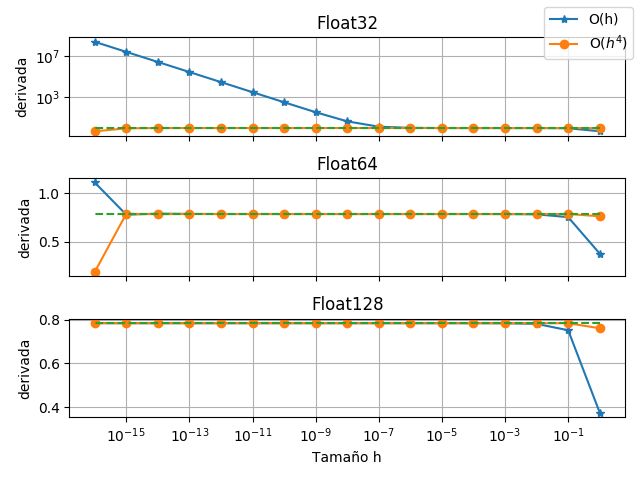
\includegraphics[height=8cm]{P1.png}
  \caption{Comparación de los dos métodos con distintos grados de precisión.}
\end{figure}

Es importante notar que el primer gráfico, a diferencia de los otros dos, tiene
 escala logarítmica y no lineal. Notamos que el método depende en gran medida
 del nivel precisión que usemos, por ejemplo, para float32, la precisión es tan
  baja, que al truncar para valores de $h$ pequeños, obtenemos divisiones por cero,
  lo que hace que nuestra aproximación esté muy lejos del valor real, pero vemos
  que para $h$ del órden de $10^{-5}$ se comporta mejor, pero el rango donde esta aproximación es fiable es muy pequeño. Por otro lado, vemos que con la aproximación propuesta
  en el enunciado esta convergencia es mucho más rápida al valor de la línea punteada. También vemos que el intervalo de $h$
  para el cual la aproximación de (1) es fiable, es siempre menor que el de la
  aproximación del enunciado, esto es un punto a considerar ya que nos dice cuánto
  cambio de resolución acepta nuestro algoritmo, lo cual es muy útil ya que si
  tenemos una función errática y una que se comporta mejor en el sentido que no
  tiene cambios de concavidad brusco y tiene derivadas pequeñas, podemos usar la
  misma función con distintos $h$ y esperar un buen resultado sin tener que hacer
  otra implementación.

  En síntesis, si usamos un número de mayor presición, logramos que el rango donde nuestra aproximación es útil, en términos de $h$ sea mucho más amplio.




\section{Pregunta 2:}

Lo primero es regularizar la integral. Para ello usamos el siguiente cambio de variable\\ $\sin\theta = \frac{\sin(\phi/2)}{\sin (\phi_/2)}} $ y $k=\sin(\phi_0/2)$, con lo que el problema se
transforma en:

\begin{equation}
  \frac{T}{T_0}=\frac{2}{\pi}\int_0^{\frac{\pi}{2}}  \frac{d\theta}{\sqrt{1-k^2 \sin^2\theta}}
\end{equation}


Al integrar para un muestreo de los $\phi_0$ indicados en el enunciado, tenemos el siguiente gráfico:




\begin{figure}[!ht]
  \centering
  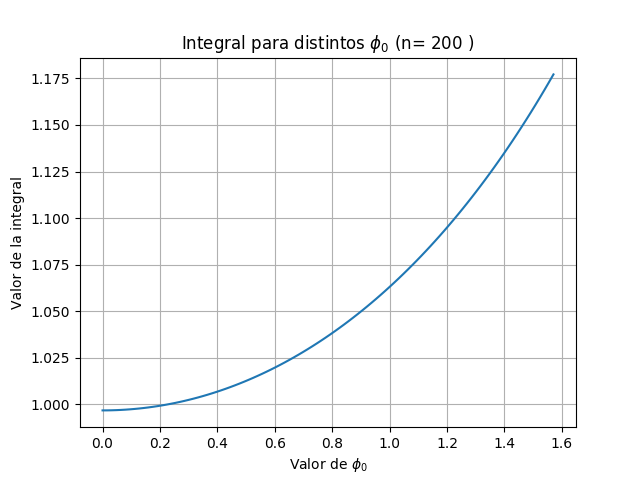
\includegraphics[height=8cm]{../informe/P2.png}
  \caption{Resultado de la integral para distintos $\phi_0$}
\end{figure}


Para lograr esto hubo que restar un poco el dominio original y restarle a $\pi/2$
un poco con la intención de evitar divisiones por cero, de todas maneras, lo que se
restó es despreciable con respecto al dominio de integración, por lo que es posible
argumentar que sigue siendo una buena aproximación para nuestro problema.

En cuanto a la velocidad de nuestra implementación, al usar \%timeit obtivimos que para la función ``Evalua'' una vuelta tarda en promedio $11.1 ms \pm 286 \mu s$
en cambio, (teniendo en cuenta que la aproximación implementada cumplió el criterio de convergencia con $n=200$, por lo que usaremos el mismo $n$ en las implementaciones de scipy) tenemos que \emph{scipy.integrate.trapz} demoró en promedio $4.38 ms \pm 218 \mu s$. Esta drástica diferencia radica en que la implementación de scipy está hecha en un lenguaje compilado, probablemente C o FORTRAN mientras que la nuestra está en uno interpretado, en este caso Python.







\section{Discusión y Conclusiones}

Podemos concluir que por un lado la presición es muy importante al resolver problemas numéricos, pero hay que tener en cuenta que hay consecuencias en la precisión y esto es la demanda computacional, ya que siempre es una aproximación y por lo mismo nos podemos dar libertades como las hechas en la pregunta 2, donde cortamos el dominio de integración para evitar problemas al evaluar la función.


\end{document}
